\documentclass{article}

% URLs and hyperlinks ---------------------------------------
\usepackage{hyperref}
\hypersetup{
    colorlinks=true,
    linkcolor=blue,
    filecolor=magenta,      
    urlcolor=blue,
}
\usepackage{xurl}
%----------------------------------------------------

\usepackage{amsmath, amssymb, empheq}
\usepackage{enumitem}
\usepackage{adjustbox}
\usepackage{euler}
\usepackage{graphicx}
\usepackage{float}

\usepackage{xepersian}
\settextfont{Yas}
\newcommand{\modts}{\overset{26}{\equiv}}

\title{تکلیف اول}
\author{مهدی حق‌وردی}
\date{\today}

\begin{document}
\maketitle
\tableofcontents

\begin{abstract}
پاسخ‌های تمرین اول به ترتیب سوالات در قالب قسمت‌‌‌‌های نام برده در فهرست نوشته شده‌اند. کدهای سوال اول در فایل \lr{zip} قرار دارند. اگر در پاسخی از منبعی استفاده شده است، لینکی از آن منبع در پانویس گذاشته شده است.
\end{abstract}

\newpage
\section{سوال اول - شکستن متن شنود شده}
متن شنود شده را با تمامی کلید‌‌های ممکن امتحان کردم و هر کدام از خروجی‌ها را بررسی کردم که به این رسیدم:
\begin{figure}[H]
\begin{center}
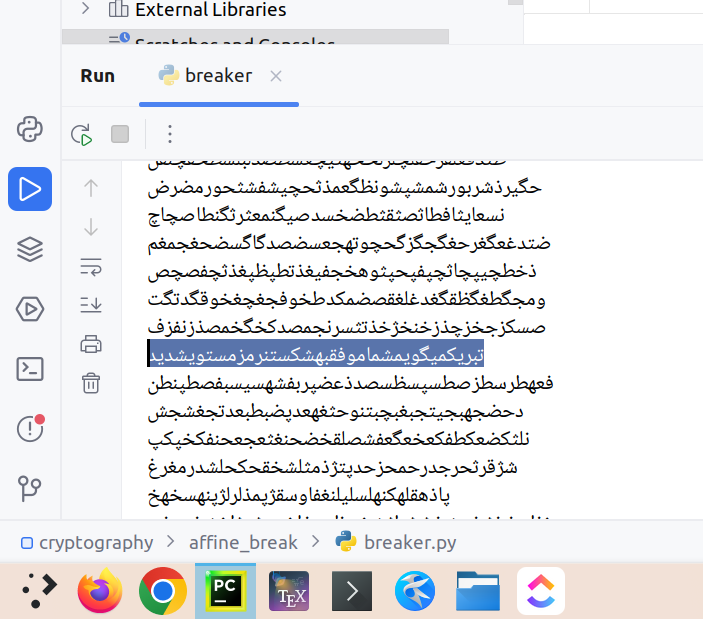
\includegraphics[width=0.63\textwidth, height=0.4\textheight]{images/found}
\end{center}
\end{figure}

\subsection{توضیحات کد}

\begin{itemize}
\item 
\lr{\texttt{pre\_needed.py}}

مقادیری که این ماژول وجود دارند مقادیری مانند الفبای فارسی، تمام کلید‌ها و یک سری ثابت هستند که در برنامه برای رمزنگاری و رمزگشایی به آنها نیاز است.

\item \lr{\texttt{functions.py}}

توابعی که در این ماژول نوشته شده‌اند دو تابع 
\lr{\texttt{encode}}
و
\lr{\texttt{decode}}
هستند که طبق فرمول‌های رمز مستوی نوشته شده‌اند.

\item \lr{\texttt{breaker.py}}

در این ماژول در حلقه‌ی 
\lr{\texttt{for}}
اول، متن رمزشده را با تمامی کلید‌های ممکن رمزگشایی کرده و نتیجه را پرینت می‌کنیم و سپس در خروجی به دنبال یک متن معنی دار می‌گردیم.

حالا برای پیدا کردن کلید هم می‌توانیم بین کلید‌ها بگردیم و آن کلیدی که متن با آن رمز شده را پیدا کنیم که آن کلید:
\lr{\texttt{Key(a=5, b=3)}}
است.
\end{itemize}


\section{شکستن رمز ویجینر با دانستن طول کلید}
\begin{enumerate}
\item 
با انجام ندادن عملیات آنالیزی

اگر نخواهیم عملیات آنالیزی روی متن رمز شده انجام دهیم، 
\lr{order}
شکستن متن رمز شده باید
$O(26^k)$
که در آن
$k$
طول کلید است را انجام داد. که در سوال
$k = 5 \Rightarrow 26^5$
می‌شود.
\LTRfootnote{from \url{https://stackoverflow.com/a/29553484/19510840}}
\item 
با انجام دادن عملیات آنالیزی

اما اگر بخواهیم باهوش باشیم و با انجام دادن عملیات آنالیزی روی متن رمز شده، آن را بشکنیم می‌توانیم با همین روش 
\lr{brute-force}
ولی با تعداد تلاش بسیار کمتری رمز را بشکنیم.

حالا که رمز ما ۵ حرف دارد، باید برای هر 
$\forall i \in \{0, 1, 2, 3, 4\}$
چنین کنیم:
\begin{equation}\label{ith}
p_i, p_{i + k}, p_{i + 2k}, p_{i + 3k},\dots
\end{equation}
انجام دهیم و متونی را از 
\lr{cipher text}
استخراج کنیم، سپس برای هر $i$ روی حروفی که این $i$ شامل می‌شود، آنالیز آماری انجام دهیم و حروفی که *ممکن* است برای کلید استفاده شده باشند را شناسایی کنیم و سپس با استفاده از تمامی جایگشت‌هایی که از حروف پیدا شده بدست می‌آیند، کلید‌ها را تک تک امتحان کنیم.

برای مثال چنین متن رمز شده‌ای داریم:

\begin{table}[H]
\begin{adjustbox}{width=\textwidth}
\begin{tabular}{c}
\lr{\texttt{PPQCAXQVEKGYBNKMAZUYBNGBALJONITSZMJYIMVRAGVOHTVRAUCTKSGDDWUOXITLAZUVAVVRAZCVKBQPIWPOU}}
\end{tabular}
\end{adjustbox}
\end{table}
و $k = 4$ داده شده است (یا از طریق روش کاسیسکی پیدا شده است.)

حالا طبق رابطه‌ی \ref{ith} برای هر یک از حروف کلید به ترتیب، متنش را استخراج می‌کنیم:

\begin{itemize}
\item $i = 0$

\begin{table}[H]
\begin{adjustbox}{width=\textwidth}
\begin{tabular}{c}
\lr{\texttt{\underline{P}PQC\underline{A}XQV\underline{E}KGY\underline{B}NKM\underline{A}ZUY\underline{B}NGB\underline{A}LJO\underline{N}ITS\underline{Z}MJY\underline{I}MVR\underline{A}GVO\underline{H}TVR\underline{A}UCT\underline{K}SGD\underline{D}WUO\underline{X}ITL\underline{A}ZUV\underline{A}VVR\underline{A}ZCV\underline{K}BQP\underline{I}WPO\underline{U}}}
\end{tabular}
\end{adjustbox}
\end{table}

که می‌شود:
\lr{\texttt{PAEBABANZIAHAKDXAAAKIU}}

و به همین ترتیب برای 
\item $i = 1$: \lr{\texttt{PXKNZNLIMMGTUSWIZVZBW}}
\item $i = 2$: \lr{\texttt{QQGKUGJTJVVVCGUTUVCQP}}
\item $i = 3$: \lr{\texttt{CVYMYBOSYRORTDOLVRVPO}} 
\end{itemize}
حالا برای هر یک از متون بدست آمده یک تحلیل آنالیزی انجام می‌دهیم و حروفی که \textbf{ممکن} است بجای آن حرف باشند را پیدا میکنیم.
برای مثال در مورد بالا چنین حروفی پیدا می‌شوند:
\begin{latin}
\begin{itemize}
\item $i = 0$ : \lr{A, I, N, W, and X} 
\item $i = 1$ : \lr{I and Z}
\item $i = 2$ : \lr{C}
\item $i = 3$ : \lr{K, N, R, V, and Y}
\end{itemize}
\end{latin}

که حالا فضای کلید‌های ما می‌شود:
$5 \times 2 \times 1 \times 5 = 50$
که بسیار بسیار کمتر از 
$26^4$
است و میتوانیم روی جایگشت‌های کلید با این حروف 
\lr{brute-force}
را اجرا کنیم.\LTRfootnote{from \url{https://inventwithpython.com/hacking/chapter21.html}}
\end{enumerate}

\section{سوال سوم}
\subsection{کلید از شماره دانشجویی}
شماره دانشجویی:
4003613023
مقدار \lr{\texttt{a}} در کلید رمز مستوی باید معکوس ضربی داشته باشد، که هم در فارسی و هم در انگلیسی عدد ۲ معکوس ضربی ندارد (چون زوج است و نسبت به ۲۶ و یا ۳۲ اول نیست.) پس دو رقم آخر شماره دانشجویی من نمی‌توانند یک کلید برای رمز مستوی باشند.

\subsection{رمزگشایی یک متن رمز شده با دو حرف آشکار}
طبق صورت سوال: $M \rightarrow P$ و 
$A \rightarrow J$
و
\begin{equation}
C_i = E_k(P_i) = aP_i + b \bmod{26}
\end{equation}
پس:
\begin{equation*}
\begin{split}
12a + b & \modts 15 \\
b & \modts 9 \Rightarrow b = 9, a = 7
\end{split}
\end{equation*}

برای محاسبه‌‌ی معکوس ضربی عدد ۷ چنین می‌کنیم:
\begin{equation*}
a^{\Phi(26) - 1} \bmod{26} \Rightarrow 7^{11} \modts 15
\end{equation*}

و حالا طبق فرمول
\begin{equation}
P_i = D_k(C_i) = (C_i - b) \times a^{-1} \bmod{26}
\end{equation}
متن رمز شده را رمزگشایی می‌کنیم:
\begin{latin}
\begin{itemize}
\item $Y = 24 \rightarrow (24 - 9)\times15 \modts 17 \rightarrow R$
\item $Z = 25 \rightarrow (25 - 9)\times15 \modts 6 \rightarrow G$
\item $Q = 16 \rightarrow (16 - 9)\times15 \modts 1 \rightarrow B$
\item $L = 11 \rightarrow (11 - 9)\times15 \modts 4 \rightarrow E$
\item $S = 18 \rightarrow (18 - 9)\times15 \modts 5 \rightarrow F$
\item $A = 0 \rightarrow (0 - 9)\times15 \modts 21 \rightarrow V$
\item $P = 15 \rightarrow (15 - 9)\times15 \modts 12 \rightarrow M$
\item $J = 9 \rightarrow (9 - 9)\times15 \modts 0 \rightarrow A$
\end{itemize}
\end{latin}
پس متن اصلی:
\lr{\texttt{RGBEFVMA}}
بوده است.

\section{معکوس ماتریس در $\mathbb{Z}_{26}$}
\subsection{$2x2$}
ماتریس معکوس 
$A = 
\begin{pmatrix}
2 & 5 \\
9 & 5 \\
\end{pmatrix}$
را در پیمانه‌ی ۲۶ بدست آورید.

\begin{equation*}
A = 
\begin{pmatrix}
2 & 5 \\
9 & 5 \\
\end{pmatrix} \Rightarrow 
C = 
\begin{pmatrix}
5 & -9 \\
-5 & 2 \\
\end{pmatrix} \Rightarrow 
\mathrm{adj}(A) = 
\begin{pmatrix}
5 & -5 \\
-9 & 2 \\
\end{pmatrix} 
\end{equation*}

\begin{equation*}
\mathrm{det}(A) = (2\times5) - (9\times5) = -31 \modts 17 \rightarrow 17^{-1} = 23
\end{equation*}

\begin{equation*}
\mathrm{det}(A)^{-1} \cdot \mathrm{adj}(A) = 
\begin{pmatrix}
23\times5 & 23\times(-5) \\
23\times(-9) & 23\times2 \\
\end{pmatrix} \Rightarrow 
A^{-1} = 
\begin{pmatrix}
11 & 15 \\
1 & 20 \\
\end{pmatrix}
\end{equation*}

\subsection{$3x3$}
ماتریس معکوس 
$A = 
\begin{pmatrix}
1 & 11 & 12 \\
4 & 23 & 2 \\
17 & 15 & 9 \\
\end{pmatrix}$
را در پیمانه‌ی ۲۶ بدست آورید.

\begin{equation*}
\begin{split}
A = 
\begin{pmatrix}
1 & 11 & 12 \\
4 & 23 & 2 \\
17 & 15 & 9 \\
\end{pmatrix} & \Rightarrow 
C = 
\begin{pmatrix}
+ \begin{vmatrix}
23 & 2 \\
15 & 9 \\
\end{vmatrix}&
- \begin{vmatrix}
4 & 2 \\
17 & 9 \\
\end{vmatrix}&
+ \begin{vmatrix}
4 & 23 \\
17 & 15 \\
\end{vmatrix} \\
- \begin{vmatrix}
11 & 12 \\
15 & 9 \\
\end{vmatrix}&
+ \begin{vmatrix}
1 & 12 \\
17 & 9 \\
\end{vmatrix}&
- \begin{vmatrix}
1 & 11 \\
17 & 15 \\
\end{vmatrix} \\
+ \begin{vmatrix}
11 & 12 \\
23 & 2\\
\end{vmatrix}&
- \begin{vmatrix}
1 & 12 \\
4 & 2 \\
\end{vmatrix}&
+ \begin{vmatrix}
1 & 11 \\
4 & 23 \\
\end{vmatrix}\\
\end{pmatrix} \\
& \Rightarrow C = 
\begin{pmatrix}
21 & 24 & 7 \\
3 & 13 & 16 \\
6 & 20 & 5 \\
\end{pmatrix} \\
& \Rightarrow \mathrm{adj}(A) = 
\begin{pmatrix}
21 & 3 & 6 \\
24 & 13 & 20 \\
7 & 16 & 5 \\
\end{pmatrix} \\
\end{split}
\end{equation*}

\begin{equation*}
\begin{split}
\mathrm{det}(A) & = 
(1 \times 
\begin{vmatrix}
23 & 2 \\
15 & 9 \\
\end{vmatrix}
) + (
-11 \times 
\begin{vmatrix}
4 & 2 \\
17 & 9 \\
\end{vmatrix}
) + (
12 \times 
\begin{vmatrix}
4 & 23 \\
17 & 15 \\
\end{vmatrix}
) \\
& = (1 \times 21) + (-11 \times 2) + (12 \times 7) = 83 \modts 5 \rightarrow 5^{-1} = 21
\end{split}
\end{equation*}

\begin{equation*}
\mathrm{det}(A)^{-1} \cdot \mathrm{adj}(A) =
\begin{pmatrix}
21\times21 & 21\times3 & 21\times6 \\
21\times24 & 21\times13 & 21\times20 \\
21\times7 & 21\times16 & 21\times5 \\
\end{pmatrix} \Rightarrow 
A^{-1} = 
\begin{pmatrix}
25&11&22\\
10&13&4\\
17&24&1\\
\end{pmatrix}
\end{equation*}

\end{document}